\section{Preliminary}\label{sec:preliminary}

\rev{Before discussing the system design for neural network acceleration, we first introduce the basic concepts of neural networks and the basic components of an FPGA-based accelerator design.}

\subsection{Neural Network}

\begin{figure}[ht]
    \centering
    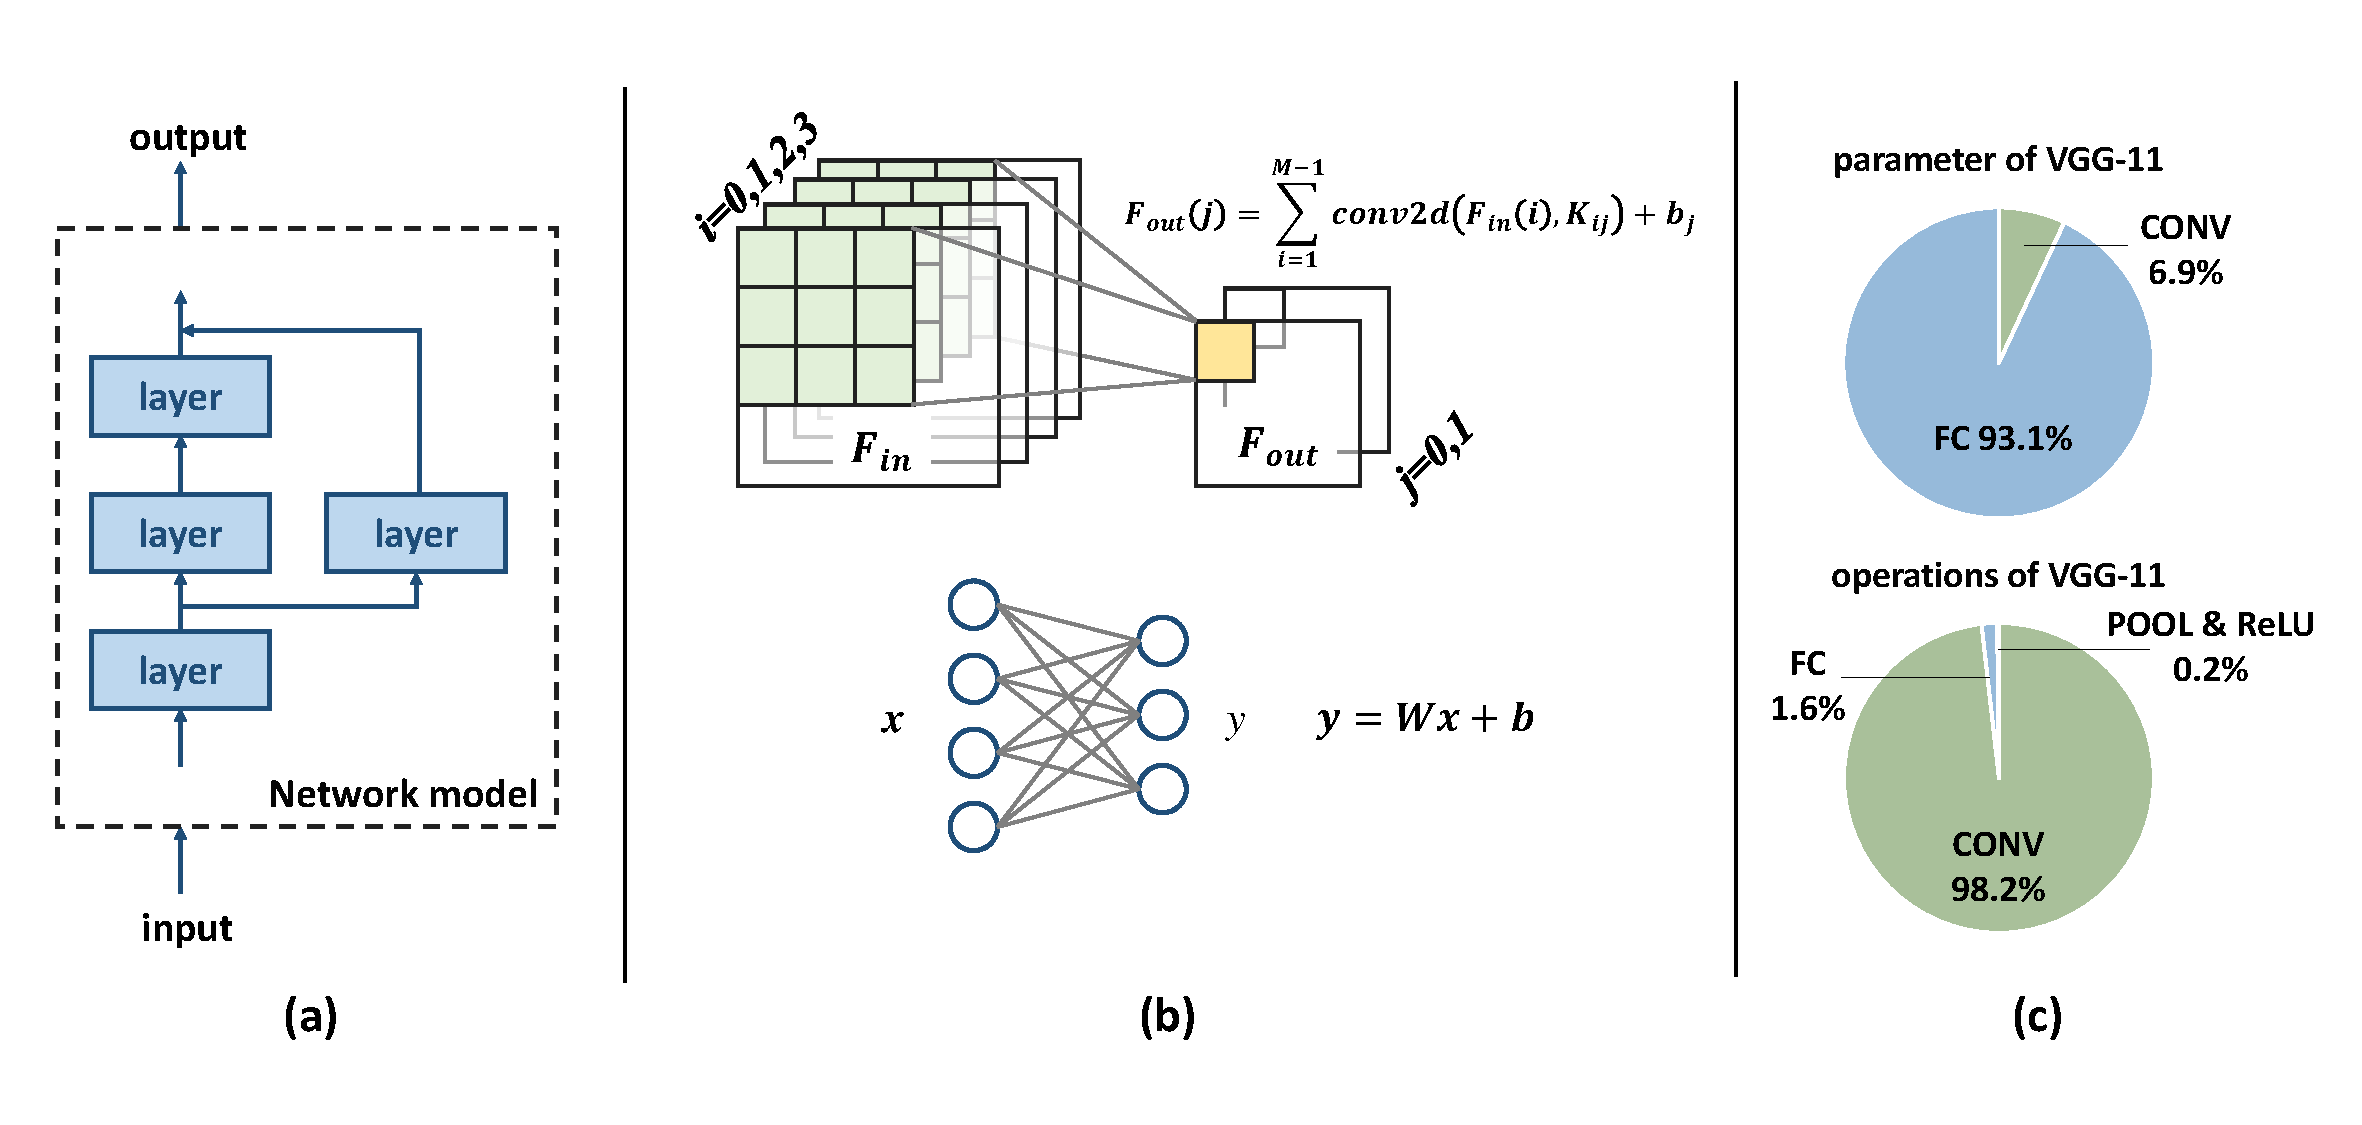
\includegraphics[width=1.0\columnwidth]{fig/cnn_preliminary.pdf}
    \caption{(a) Computation graph of a neural network model. (b) CONV and FC layers in NN model. (c) CONV and FC layers dominates the computation and parameter of a NN model.}
    \label{fig:cnn_preliminary}
\end{figure}

\rev{In this section, we introduce the basic functions in a neural network. A neural network model can be described as a directed graph shown in Figure~\ref{fig:cnn_preliminary}(a). Each vertex of the graph denotes a layer which conducts operations on data from a previous layer or input and generates results to the next layer or output.

Convolution (CONV) layers and fully connected (FC) layers are two common types of layers in NN models. The functions of these two layers are shown in Figure~\ref{fig:cnn_preliminary}(b). CONV layers conduct 2D convolutions on a set of input feature maps $F_{in}$ and add the results to get output feature maps $F_{out}$. FC layers receives a feature vector as input and conduct matrix-vector multiplications.
}

\subsection{FPGA-based Accelerator}

\rev{}

In this section, we introduce the basic operations included in neural network algorithms. Neural network is a bio-inspired model, which usually includes several layers of $neuron$. Each layer receives the neurons of the previous layer as input. In a basic neural network layer, each neuron of this layer calculates a weighted sum of all the input neurons connected to it. The weight of the connections are referred to as $weights$ in this paper. Other types of layers are also introduced in state-of-the-art neural network models. In the rest part of this section, we introduce different types of layers.

{\bf{Fully conencted (FC) layer}} implements a connection between every input neuron and output neuron with a weight. This type of layer is adopted in both CNN and RNN. The input and output neurons of an FC layer are two vectors $\bf{x}$ and $\bf{y}$. The weights of this layer can be modeled as a matrix $W$. A bias vector $b$ is added to each of the output neuron. The function of this layer is described as equation.
\begin{equation}\label{eqt:fc}
    {\bf{x}} = W{\bf{y}} + {\bf{b}}
\end{equation}

{\bf{Convolution (CONV) layer}} is used for 2-d neuron process. This is commonly adopted in CNN for image process. The input and output neurons of this layer can be described as sets of 2-d feature maps, $F_{in}$ and $F_{out}$. Each feature map is called a channel. A CONV layer implements a 2-d convolution kernel $K_{ij}$ for each input and output channel pair and a bias scalar $b_i$ for each output channel. The computation of a CONV layer with $M$ input channels and $N$ output channels can be described as equation~\ref{eqt:conv}.
\begin{equation}\label{eqt:conv}
    F_{out}(j) = \sum_{i=0}^{M-1} \text{conv2d}(F_{in}(i), K_{ij}) + b_j \qquad j=0,1,...,N-1
\end{equation}
There are varieties of 2-d convolutions in CONV layer. Usually standard convolution with padding is used when the kernel size is $3\times 3$. For larger kernels like $5\times 5$ and $7\times 7$, a stride larger than 1 is usually used to reduce the number of operation and feature map size. Recent work is also using $1\times 1$ convolution kernels~\cite{he2016deep, iandola2016squeezenet}.

{\bf{Non-linear layer}} applies a non-linear function on each of the input neurons. Sigmoid function and tanh function are commonly adopted in early models and are still used in RNN for acoustic or speech recognition. Rectified linear unit (ReLU)~\cite{krizhevsky2012imagenet} is the adopted in many state-of-the-art models. This function maintains the positive neurons and filters negative neurons as zero. Varieties of ReLU are also used, such as PReLU and Leaky ReLU~\cite{xu2015empirical}.

{\bf{Pooling layer}} is also used for 2-d neuron process like CONV layer. A pooling layer downsamples each of the input channel respectively, which helps reduce feature dimension. There are two kinds of down sampling method: average pooling and max pooling. Average pooling splits a feature map into small windows, i.e. $2\times2$ windows, and finds the average value of each window. Max pooling method finds the maximum value in each window. Common window size includes $2\times2$, stride=2 and $3\times3$, stride=2.

{\bf{Element-wise layer}} is usually used in RNN and is also introduced in some CNN models like \cite{he2016deep}. This layer receives two neuron vectors of the same size and applies element-wise operations on corresponding neurons of the two vectors. In ResNet, this layer is element-wise addition. For RNN, this layer can be element-wise subtraction or multiplication.

Among these types of layers, FC layer and CONV layer contributes to most of the computation and storage in neural networks. In the following sections, both software level and hardware level designs focus on these two types of layers.